\documentclass[12pt, a4paper]{article}

\usepackage{authblk}
\usepackage[utf8]{inputenc}
\usepackage[T2A]{fontenc}
\usepackage[serbianc]{babel}
\usepackage{hyperref}
\usepackage{amsmath}
\usepackage{graphicx}

\renewcommand\Authsep{\par}
\renewcommand\Authands{\par}

\title{Увод у каузално (узрочно) закључивање}
\author{Александра Новаковић 368/22}
\author{Милица Ињац 338/18}
\author{Бојан Корда 121/19}
\affil{Математички факултет, Универзитет у Београду}
\date{\today}

\begin{document}
\maketitle
\newpage

\tableofcontents
\newpage

\section{Фундаментални проблем}
\subsection{Увод}
У многим применама статистике, велики део истраживачких питања заправо је питање каузалности, а не само описивања података или испитивања њихове повезаности.
На пример, медицински истраживач може желети да утврди да ли је нови лек заиста ефикасан у лечењу одређене болести. Економиста може бити заинтересован за 
испитивање ефеката програма обуке на запосленост појединаца, док социолог може проучавати како развод родитеља утиче на даљу едукацију деце. 
У свим овим примерима циљ је да се утврди узрочни однос између одређене интервенције и исхода, а не само да се опишу обрасци у подацима.

За разлику од пуке корелације, каузално закључивање тежи да одговори на питање: \textit{„Шта би било, кад би било?“} Ову идеју можемо јасније приказати на примеру из 
филма „Диван живот“, у којем главни лик, Џорџ Бејли, пролази кроз дубоку кризу и тврди да би свет био боље место да се он никада није родио. У том тренутку појављује 
се анђео који му показује како би свет изгледао у контрафактуалном сценарију — свету у којем Џорџ није постојао. У том свету, између осталог, његова деца никада нису 
рођена, његов млађи брат умире као дете јер није било никога да га спаси, а фармацеут погрешно издаје рецепт и бива осуђен за убиство из нехата. Супротстављањем 
стварног света (у којем је Џорџ присутан) и контрафактуалног света (у којем га нема), филм сликовито приказује суштину каузалног закључивања: поређење између онога 
што јесте и онога што би могло да буде.

Идеја каузалног закључивања заснива се на поређењу стварно посматраног исхода са потенцијалним исходима који би се могли догодити да је третман био другачији. 
Међутим, проблем је у томе што те алтернативне исходе никада не можемо посматрати директно — они су контрафактуални. Због тога се каузално закључивање у 
основи може посматрати као проблем са недостајућим подацима: од кључног значаја је механизам који одређује који подаци су посматрани, а који не. У контексту 
каузалне анализе, овај механизам назива се механизам доделе третмана, јер одређује који ентитети добијају који ниво третмана.

Ово поглавље и следеће баве се каузалним закључивањем, које се односи на питање шта би се догодило са неким исходом $y$ као резултат хипотетичког третмана.
У оквиру регресионог модела, третман се може представити променљивом $T$:
$$
T_i =
\begin{cases}
1, & \text{ако јединица} i \text{добије третман},\\
0, & \text{ако јединица} i \text{припада контролној групи}
\end{cases}
$$
а у случају континуираног третмана, $T_i$ представља ниво третмана који је додељен јединици $i$.

У уобичајеном регресионом контексту, предиктивно закључивање се односи на поређења између различитих јединица, док се каузално закључивање бави 
поређењем различитих третмана који би били примењени на исту јединицу. Уопштено посматрано, каузално закључивање се може сматрати посебним случајем предикције, 
у којем је циљ да се предвиди шта би се догодило под различитим опцијама третмана.

Коришћење контролисаних студија представља најефикаснији начин за утврђивање узрочних веза између променљивих. У контролисаној студији, узорак или популација 
се дели на две групе које су међусобно упоредиве по скоро свим карактеристикама. Након тога, групе добијају различите третмане, а њихови исходи се посебно 
анализирају и упоређују.

\subsubsection{корелација не повлачи узрочност}
Каузалност је област статистике која се често погрешно разуме и неправилно примењује због уверења да, ако подаци показују корелацију, 
нужно постоји и узрочна веза иза тога.

Када петао запева, убрзо након тога сунце излази — али знамо да петао није узрок изласка сунца. Да је петла појео сеоски мачак, сунце би ипак свануло.
У једној студији индустрија чоколаде је тврдила да „конзумирање чоколаде производи Нобелове лауреате“. Иако би конзумација чоколаде могла утицати на повећање броја 
Нобелових лауреата, обрнуто је такође могуће — повећање броја лауреата могло је довести до повећане потрошње чоколаде, нпр. због прослава. Вероватније је да 
непосматране променљиве, као што су социо-економски статус или квалитет образовног система, могу истовремено утицати и на потрошњу чоколаде и на број лауреата, чиме 
је корелација између њих неузрочна. 

\begin{figure}[h!]
    \centering
    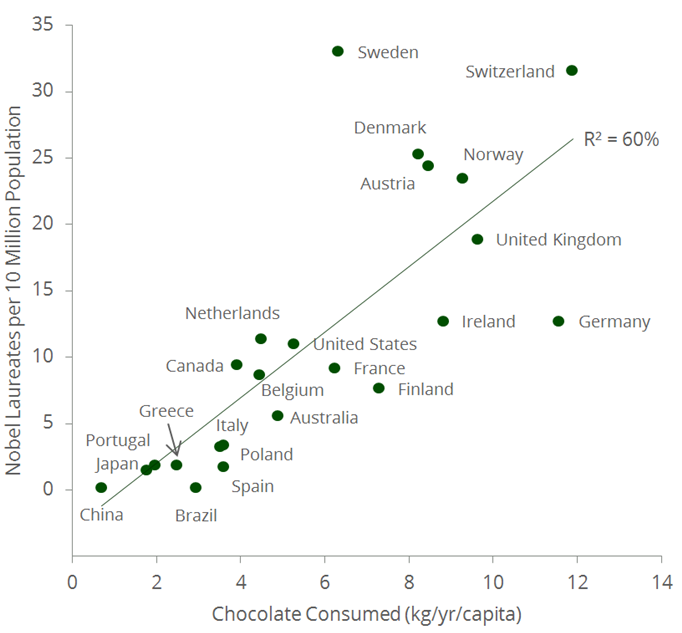
\includegraphics[width=0.7\textwidth]{Chocolate_consumption.png}
    \caption{Конзумација чоколаде и добитници Нобелове награде. Преузето са: \textit{https://www.dectech.co.uk/news-insights/buzz/why-is-correlation-not-causation-part-i/}}
    \label{fig:uzrocnost}
\end{figure}

Да бисмо избегли оваква погрешна тумачења, важно је јасно разграничити шта је корелација, а шта каузалност и разумети на који начин се ови односи испитују у статистици.

Корелација и каузалност представљају две различите врсте односа између променљивих. Корелација описује статистичку повезаност: две променљиве се крећу заједно на 
предвидљив начин, али то не значи да промена једне узрокује промену друге. Каузалност, с друге стране, подразумева да промена једне променљиве директно доводи до 
промене друге, при чему постоји стварна узрочна веза. Док корелација мери само обрасце заједничког кретања података, каузалност захтева разумевање механизма који 
повезује променљиве и обично укључује контролу других фактора који могу утицати на посматрани однос.

Корелација представља најнижи ниво каузалне хијерархије и дефинише се поређењем очекиваног исхода код тренираних и нетретираних у стварном свету, $E[Y|A=1] \neq E[Y|A=0]$.
Каузалност подразумева поређење целокупне популације када би сви били третирани, $E[Y^{a=1}]$, са исходом када би сви били нетретирани, $E[Y^{a=0}]$.
Корелација може постојави чак и када међу њима нема каузалне везе, обично због постојања заједничког узорка.
Принцип заједничког узрока формализује ове могућности: ако су две случајне променљиве $X$ и $Y$ статистички 
зависне, онда је могуће да 
\begin{enumerate}
    \item $X$ узрокује $Y$
    \item $Y$ узрокује $X$
    \item постоји трећа променљива $Z$ која узрокује и $X$ и $Y$, при чему $X$ и $Y$ постају независне ако се узме у обзир $Z$
\end{enumerate}
Каузално закључивање пружа алате који нам омогућавају да донесемо узрочне закључке чак и у одсуству истинског експеримента, под условом да су испуњене
одређене претпоставке (условна заменљивост, позитивност и конзистентност) о којима ће бити речи касније. 

Да би се боље разумела практична важност каузалног закључивања, корисно је погледати како оно функционише у стварним истраживачким ситуацијама и како помаже да се 
избегну погрешни закључци засновани само на корелацији.

\subsubsection{Главне разлике, истраживања, илустрација примером}
Каузално закључивање је важно, на пример, у медицинским истраживањима једна група може добијати плацебо, док друга добија нови тип лека.
Ако се исходи између те две групе значајно разликују, управо различита искуства могу бити узрок тих различитих исхода.

Поред експерименталних дизајна, каузално размишљање је кључно и код анализа опсервационих података. Један од феномена који најбоље илуструје ову потребу јесте 
Симпсонов парадокс.

Симпсонов парадокс представља појаву у којој се однос између две променљиве мења или чак потпуно преокреће када се подаци 
посматрају у целини у односу на њихове подгрупе. Другим речима, корелација која важи на агрегатном нивоу може нестати или 
се обрнути када се подаци разбију по релевантним категоријама.

Овај парадокс јасно показује зашто „корелација не повлачи узрочност“ – наизглед јака веза може бити последица прикривених 
(конфаундирајућих) фактора. %ovde dodati i primer sa doktorima
Класичан пример је анализа успеха лечења код мушкараца и жена: када се посматрају подаци укупно, 
једна терапија делује успешније, док када се подаци раздвоје по полу, испостави се да је друга терапија боља у обе групе.

Суштина Симпсоновог парадокса је у томе да исту корелацију можемо тумачити потпуно другачије у зависности од нивоа анализе. 
Због тога се у каузалном закључивању наглашава важност идентификације и контроле скривених променљивих како би се избегли 
погрешни закључци.

Разликовање корелације и каузалности је само први корак ка разумевању узрочних односа. Да бисмо могли прецизније да објаснимо и измеримо ефекте различитих интервенција, 
потребан нам је формалнији оквир. У наставку ће бити представљени кључни појмови као што су контрафактуални исходи, просечни третмански ефекат (ATE), претпоставка 
SUTVA и Рубинов каузални модел, који нам помажу да каузално размишљање претворимо у конкретне статистичке алате.


\subsection{Фундаментални проблем}
    \subsubsection{Рубинов каузални модел}

Фундаментални проблем каузалног закључивања, како га је назвао Пол Холанд 1986. године, чињеница да за сваку појединачну јединицу (особу, објекат) која је 
предмет истраживања може бити посматран само један од два потенцијална исхода. То значи да не можемо истовремено посматрати шта се дешава са једним појединцем након 
што је примио третман (нпр. $T=1$) и шта се дешава са тим истим појединцем након што није примио третман (нпр. $T=0$), у истом тренутку. Другим речима, каузални ефекат 
на индивидуалном нивоу увек остаје делимично непознат, јер је један од исхода нужно контрафактуалан (непосматран, хипотетички исход, супротан посматраним чињеницама).
Због ове немогућности истовременог посматрања, никада не можемо директно измерити индивидуални каузални ефекат.

Доналд Рубин је 1974. године формализовао овај проблем и увео основни језик за кодирање каузалности. Овај модел назива се Рубинов Каузални Модел (РЦМ), састоји се 
из три градивна блока, кључних за дефинисање каузалног ефекта.
\begin{enumerate}
    \item \textbf{Потенцијални исходи} За сваку јединку $i$, дефинишу се два потенцијална исхода, $Y_i^1$ или $Y_i^0$ у зависности од тога да ли 
    је јединка примила третман ($T_i=1$) или није ($T_i=0$). Пре доношења одлуке о додели третмана, оба ова стања су теоретски изводљива за сваку јединку па се каузални 
    ефекат дефинише као разлика потенцијалних исхода, односно $\Delta^Y_i = Y_i^1 - Y_i^0$.
    \item \textbf{Правило доделе третмана} То је променљива $D_i$ која одлучује ко прима третман ($Т_i=1$) и ко остаје у контролној групи ($Т_i=0$). Правило 
    доделе је кључно јер одређује који од два потенцијална исхода ће бити посматран. Механизам додељивања третмана је важан јер утиче на очекиване вредности потенцијалних исхода.
    \item \textbf{Једначина преклапања, прекидна једначина} Ова једначина повезује посматрани исход $Y_i$ са потенцијалним исходима, преко променљиве $D_i$: $Y_i = D_i Y^1_i + (1 - D_i) Y^0_i$.
    Оне објашњава да посматрамо само исход који одговара третману који је заиста примљен.
\end{enumerate}
РЦМ је, у суштини, модел о делимично посматраним случајним варијаблама па се каузално закључивање може посматрати као предвиђање шта би се догодило са јединицом $i$ 
ако би $D_i=0$ или $D_i=1$.

Да би потенцијални исходи били добро дефинисани, неопходна је претпоставка о стабилној вредности третмана јединице (\textit{eng. Stable Unit Treatment Value Assumption, SUTVA}), 
која подразумева да исход једне јединке не зависи од третмана других и да не постоје скривене варијанте третмана. 
Na primer, ishod jedne osobe koja prima transplantaciju srca ne bi trebalo da zavisi od toga da li je i druga osoba primila transplantaciju.
npr. različiti hirurzi, procedure, oprema

Како индивидуални ефекти нису директно доступни, у пракси се користе користе агрегатне мере каузалног ефекта, попут просечног ефекта третмана 
(\textit{eng. Average Treatment Effect, ATE}), $\theta = E{Y_i(1)} - E{Y_i(0)}$, или просечног ефекта на третиране (\textit{eng. Average Treatment Effect on the Treated, ATT}), 
$\Delta^Y_{TT} = E{Y_i^1 - Y_i^0 | D_i=1}$. Ове мере омогућавају поређење група и дају емпиријски смисао истраживањима у којима се тражи процена узрочних утицаја. Да би 
се ови просечни ефекти могли проценити, поред СУТВА, потребне је и кључна статистичка претпоставка о јакој игнорабилности, која укључује:
\begin{itemize}
    \item \textbf{Неконфузност} Потенцијални исходи су независни од доделе третмана, условљено коваријатама\footnote{Предтретмантске контролне променљиве $X_i$ су све оне које су посматране или мерене 
пре него што је јединка примила третман. Служе као улазни подаци у регресионим моделима ради постизања условне заменљивости између третиране и контролне групе.}:
$$
(Y^1_i, Y^0_i) \perp D_i | X_i
$$
Ово значи да је, унутар слојева дефинисаних коваријатама, третман насумично додељен. Неконфузност је од суштинског значаја за елиминисање пристрасности услед селекције и посебно 
је важна у опсервационим студијама.
    \item \textbf{Позитивност} За сваку комбинацију вредности коваријата $X$, постоји ненула вероватноћа да ће јединица примити и третман и контролу:
$$
0 < Pr(D_i=1|X_i=x) < 1
$$
У случају кршења ове претпоставке, просечан каузални ефекат не може бити процењен ни са бесконачном количином података. Позитивност је кључна за методе засноване на 
вероватноћи третмана(\textit{eng. Propensity Score}), јер се условна средња вредност не може дефинисати ако је вероватноћа примања третмана, за дату комбинацију коваријата, једнака нули.
\end{itemize}

У практичном контексту, ATE омогућава да проценимо колики би био очекивани ефекат третмана када би се применио 
на целу циљну групу, јер се у друштвеним, биомедицинским и економским истраживањима ретко усредсређујемо на индивидуалне ефекте. 
Уместо тога, истраживаче углавном занима просечан утицај третмана на популацији, што има директне импликације за 
креирање јавних политика, медицинске интервенције или економске мере.

Ипак, ATE има и одређена унутрашња ограничења која је важно разумети приликом њене интерпретације:
\begin{enumerate}
    \item \textbf{Неидентификованост индивидуалних ефеката:}
Како индивидуални ефекти нису директно доступни, ATE се односи на просечан каузални ефекат у популацији, а не на појединачне јединице.
    \item \textbf{Прикривање хетерогености ефеката:}
Како АТЕ представља просек ефекта у популацији, она може прикрити значајне разлике међу појединцима или подгрупама. На пример, ако третман једнако помаже 
једној половини популације, а одмаже другој, просечни ефекат може бити нула, иако су индивидуални ефекти изражени и хетерогени.
    \item \textbf{Зависност од карактеристика популације:}  
Величина ATE-а зависи од дистрибуције индивидуалних ефеката у посматраној популацији. Ако одређени фактори (нпр. пол, старост или социоекономски статус) модификују 
ефекат третмана, ATE ће се разликовати између популација са различитом структуром ових фактора. Стога, ова мера није нужно стабилна при преношењу резултата на друге 
популације.
    \item \textbf{Зависност од претпоставки и механизма доделе третмана:}  
Процена ATE-а у великој мери почива на претпоставкама о начину доделе третмана и о одсуству конфаундерa. Уколико третман није насумично додељен и ако нису 
задовољене кључне претпоставке попут неконфузности и позитивности, процене ATE-а могу бити пристрасне.
    \item \textbf{Предиктивни, а не објашњавајући карактер:}  
Каузално закључивање се може посматрати као предвиђање онога што би се догодило јединки $i$ под различитим условима третмана, стога ATE даје просечну предикцију за 
целу популацију.
\end{enumerate}

С обзиром на наведена ограничења, процена ATE-а у пракси захтева пажљиво осмишљене статистичке приступе који омогућавају да се „реконструишу” недостајући 
контрафактуални исходи. Циљ ових метода је да, под одређеним претпоставкама, омогуће непристрасну и 
поуздану процену просечних ефеката третмана. У зависности од контекста истраживања и начина доделе третмана, користе се различите стратегије као што су 
регресиони естиматори, методе засноване на вероватноћи доделе третмана, метода упаривања јединица са сличним карактеристикама. Све ове методе имају 
заједнички циљ: да обезбеде што бољу апроксимацију контрафактуалних исхода и тиме омогуће валидно каузално закључивање.

Да бисмо илустровали различите начине процене просечног каузалног ефекта третмана (ATE), у наставку ћемо упоредити више приступа на истом симулираном примеру.
Размотрена су два сценарија: у првом, додела третмана је насумична и независна од коваријата, док у другом зависи од предтретманских карактеристика (постоји конфаундинг).
На слици приказујемо поступак упаривања јединица са сличним предтретманским карактеристикама — за сваку третираној јединицу проналази се најсличнија контролна 
јединица према процењеној вероватноћи доделе третмана, након чега се израчуната разлика у просечним исходима користи као приближна процена ATE-а.

У случају насумичне доделе, наивна разлика у срединама, регресиони модел и упаривање дају приближно исте резултате, што потврђује да није неопходна сложенија метода када 
су групе по дефиницији упоредиве. Међутим, када додела третмана зависи од коваријата, наивна процена постаје пристрасна — у том случају методе које контролишу за 
конфаундере (регресиони модели или упаривање) омогућавају добијање процене ближе стварном ATE-у.  (Verovatno jer je sample relativno mali, X1 utiče jako na verovatnoće tretmana, pa se za neke tretirane jedinice ne nalaze dobri kontrolni parovi → dolazi do pristrasnosti i veće varijanse.
U teoriji, matching je konzistentan ako su pretpostavke zadovoljene)


Процена ATE-а и илустрација приближавања контрафактуалних исхода указују на ограничења једноставних просечних ефеката и потребу за методама које контролишу доделу 
третмана и конфаундере. У наредним деловима рада разматраћемо рандомизоване експерименте, где насумична додела минимизује проблем контрафактуалности, и опсервационе 
студије, које се ослањају на статистичке приступе за валидну процену каузалних ефеката.


%Да би концепт приближавања недостајућих контрафактуалних исхода био јаснији, у наставку представљамо једноставни пример који користи упаривање по вероватноћама доделе. 
%Слика приказује како се третиране јединице пореде са контролним јединицама сличних предтретмантских карактеристика, а разлика у просечним исходима приближно 
%представља ATE. 


%Овај пример служи као илустрација концепта и увод у практичне методе процене каузалних ефеката, без претензије 
%на емпиријски значај.

%Процена ATE-а и илустрација приближавања контрафактуалних исхода указују на ограничења једноставних просечних ефеката и потребу за методама које контролишу доделу 
%третмана и конфаундере. У наредним деловима рада разматраћемо рандомизоване експерименте, где насумична додела минимизује проблем контрафактуалности, и опсервационе 
%студије, које се ослањају на статистичке приступе за валидну процену каузалних ефеката.

%Тако дефинисано, процена ATE-а представља само један део ширег оквира каузалног закључивања. У наредним деловима рада фокусираћемо се на конкретне приступе који се 
%користе за процену каузалних ефеката у различитим контекстима: прво ћемо размотрити рандомизоване експерименте, који омогућавају директну контролу доделе третмана и 
%минимизирају проблем контрафактуалности, а затим ћемо се осврнути на опсервационе студије, у којима се процене ATE-а ослањају на статистичке методе и претпоставке за 
%контролу конфаундера.

    \subsubsection{АТЕ (Average Treatment Effect), дефиниција}
    \subsubsection{проблем контрафактуала, немогућност да посматрамо оба света истовремено}
\subsection{Математичке основе иза концепта узрочности}
    \subsubsection{АТЕ (процена и математичке импликације)}
    \subsubsection{СУТВА}
    \subsubsection{алгоритми за процену ефекта}
\subsection{Утврђивање кауланости и експерименти (прелазак на следеће поглавље)}

\newpage



\section{Рандомизирани експеримент}
\newpage



\section{Опсервационе студије}


\end{document}

